\documentclass[slovene,11pt,a4paper]{article}
\usepackage[margin=1.8cm,bottom=3cm,foot=1.5cm]{geometry}
\usepackage{amsmath}
\usepackage{booktabs}
\usepackage{float}
\usepackage{graphicx}
\usepackage{gensymb}
\usepackage{geometry}
\usepackage{changepage}
\usepackage{subcaption}
\usepackage{multirow}
\usepackage{blindtext}
\usepackage{hyperref}
\usepackage[version=4]{mhchem}
\usepackage[slovene]{babel}
\pagenumbering{gobble}
\renewcommand{\contentsname}{\centering Contents}

\begin{document}

\title{6. naloga - Luščenje modelskih parametrov in različni modeli}
\author{Tadej Lozej 28201055}
\maketitle
\begin{center}
Modelska analiza 1 \\
\bigskip
Predavatelj: prof. dr. Simon Širca \\
Asistent: doc. dr. Miha Mihovilovič
\end{center}

\newpage

\tableofcontents

\newpage

\section{Uvod}

\pagenumbering{arabic}

Naša naloga je prilagajanje funkcij izmerjenim vrednostim in določanje parametrov prilagojenih funkcij. Obravnavali bomo model vezave reagenta na receptor v tkivu, delovanje ledvic in rekonstrukcijo trajektorije delcev v magnetnem spektrometru. Pri reševanju bomo uporabljali funkcijo \texttt{curve\_fit} iz modula \texttt{scipy.optimize} v programskem jeziku \texttt{Python}. Ustreznost prilagojene funkcije $f(x, \vec{a})$ s parametri $\vec{a}$ bomo preverjali s testom reducirani $\chi^2$, ki ga izmedemo s funkcionalom

\begin{equation}
\chi^2 = \frac{1}{N-M} \sum_{i=1}^n \left[
\frac{y_i - f(x_i, \vec{a})}{\sigma_i}
\right]^2,
\end{equation}
kjer je $N$ število izmerkov in $M$ število parametrov prilagojene funkcije.

\section{Farmakologija}

V farmakologiji nerijo odziv tkov na različne reagente. Za večino teh pojavov lahko privzamemo, da gre za reakcijo, kjer spremljamo vezavo molekul reagenta $X$ na receptorje $Y$ v tkivu

\begin{equation}
\ce{Y+X <=> Y^*}.
\end{equation}

\subsection{Linearni model}

V stacionarnem stanju dobimo zvezo

\begin{equation}
y = \frac{y_0 x}{x+a}.
\end{equation}
Naša naloga je iz merskih podatkov v datoteki \texttt{farmakoloski.dat} določiti parametra $y_0$ in $a$, kjer pomeni $y_0$ nasičeni odziv tkova in $a$ koncentracijo, potrebno za odziv, ki je enak polovici nasičenega. Merjeni podatki so podani v tabeli 1. Napaka v meritvi odziva je v vsem področju enaka trem enotam.

\begin{table}[h!]
\centering
\begin{tabular}{ccr}
\toprule
x[doza] &  y[odziv] &  $\sigma_y$[odziv] \\
\midrule
   1 &    0.0001 &          3 \\
   2 &    0.0010 &          3 \\
   7 &   15.300 &          3 \\
  10 &   34.600 &          3 \\
  20 &   49.300 &          3 \\
  70 &   82.600 &          3 \\
 200 &   96.000 &          3 \\
1000 &  100.00 &          3 \\
\bottomrule
\end{tabular}
\caption{Podatki o prejetih dozah in odzivu iz datoteke \texttt{farmakoloski.dat}.}
\end{table}

Bolje kot da slepo prilegamo krivuljo oblike iz enačbe (3) podatkom v tabeli 1 je prvo linearizirati dobljeno zvezo in ustrezno pretvoriti podatke za linearen fit. Vidimo, da enačbo (3) lahko lineariziramo kot

\begin{equation}
Y(X) = a_1 + a_2 X,
\end{equation}
kjer je $X = 1/x$ nova neodvisna spremenljivka, $Y = 1/y$ nova odvisna spremenljivka ter $a_1 = 1/y_0$ in $a_2 = a/y_0$ nova parametra. V skladu z novimi predpisi spremenljivk moramo tudi transformirati podatke iz tabele 1, katerim bomo nato prilagajali premico. V tabeli 2 so prikazani transformirani podatki, katerim prilagajamo premico iz enačbe (4). Seveda nesmemo pozabiti na transformacijo napak merjene odvisne spremenljivke! Izkaže se, da novo napako dobimo po formuli

\begin{equation}
\sigma_{Yi} = \frac{\sigma_{yi}}{y_i^2}.
\end{equation}
Tako je smiselno, da imata najmanjša $y$ izmerka po transformaciji zelo veliko napako.

\begin{table}[h!]
\centering
\begin{tabular}{ccr}
\toprule
    X &      Y & $\sigma_{Yi}$ \\
\midrule
1.000 &  10000 &  3e+08   \\
0.500 &   1000 &  3e+06   \\
0.143 &  0.065 &  1.3e-02 \\
0.100 &  0.029 &  2.5e-03 \\
0.050 &  0.020 &  1.2e-03 \\
0.014 &  0.012 &  4.4e-04 \\
0.005 &  0.010 &  3.3e-04 \\
0.001 &  0.010 &  3.0e-04 \\
\bottomrule
\end{tabular}
\caption{Transformirani podatki o prejetih dozan in odzivu iz datoteke \texttt{farmakoloski.dat}. Na te podatke bomo prilagajali premico, ki jo določa enačba (4).}
\end{table}
\noindent Na sliki 1 vidimo prilagajanje enačba (4) podatkom iz tabele 2. Graf je prikazan v logaritemski skali zaradi iztopanja prvih dveh podatkov iz tabele 2. Njune napake sta ogromni, zato je minimizaciji enačbe reduciranega $\chi^2$ oz. enačbe (1) ne igra velike vloge. Z drugimi besedami: pri prilaganju premice ju zalo malo upoštevamo.

\begin{figure}[h!]
\centering
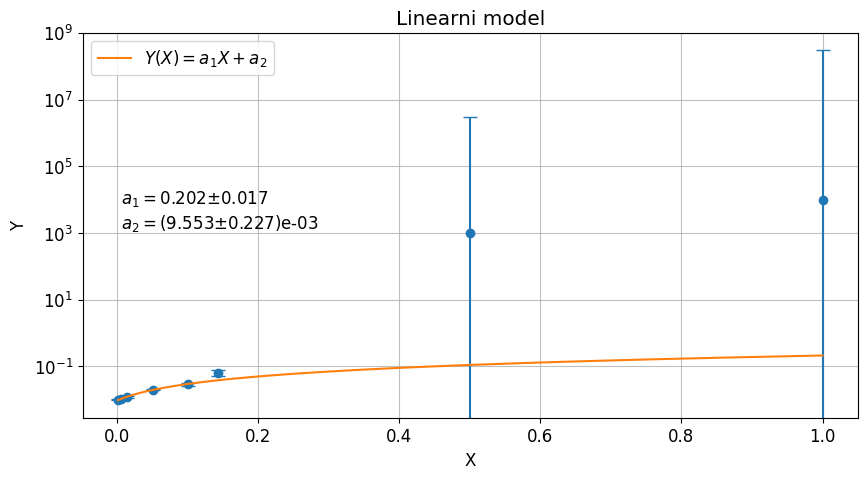
\includegraphics[width=13cm]{farma1.png}
\caption{Prilagajanje premice, ki jo določa enačba (4) podatkom iz tabele 2. Graf je prikazan v logaritemski skali zaradi iztopanja prvih dveh podatkov iz tabele 2.}
\end{figure}

Funkcija \texttt{curve\_fit} nam vrne optimalne vrednosti parametrov in kovariančno matriko. Iz kovariančne matrike lahko dobimo oceno za napako optimalnih parametrov in korelacijsko matriko. Korelacijski koeficient med dvema parametroma je definiran kot

\begin{equation}
\rho(a_j, a_k) = \frac{\text{cov}[a_j, a_k]}{\sqrt{\text{var}[a_j] \text{var}[a_k]}}.
\end{equation}
Na tak način je njegova vrednost vedno med -1 in 1. Korelacijska matrika je uporabna za ugotavljanje "varčnosti" našega fita. Če s korelacijsko matriko odkrijemo veliko korelacijo med dvema parametroma lahko enega izmed niju izločimo iz prilagojene funkcije, saj igrata v obliki funkcije podobno vlogo. Tako lahko naredimo model bolj varčen in enostaven, kar je naša želja. Na sliki 2 je prikazana korelacijska matrika v našem primeru linearnega modela. Po diagonali korelacijske matrike so seveda vrednosti 1, saj je vsak parameter sam s sabo popolno koreliran. Po enačbi (6) to tudi lahko vidimo, saj imamo v števcu in imenovalcu varianco istega parametra, kar se pokrajša v 1.

\begin{figure}[h!]
\centering
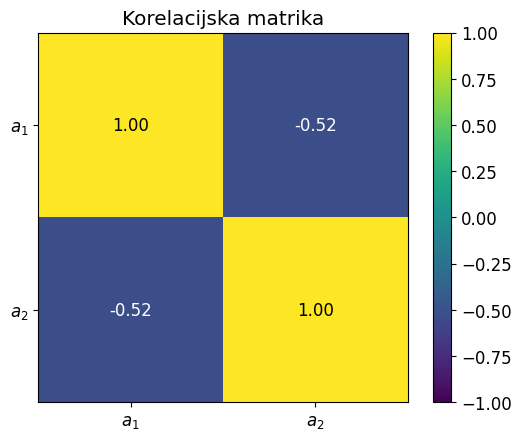
\includegraphics[width=8cm]{farma2.png}
\caption{Korelacijska matrika za parametra $a_1$ in $a_2$ pri linearnem modelu.}
\end{figure}

Iz pridobljenih parametrov $a_1$ ter $a_2$ in njunih napak lahko izračunamo iskana parametra $y_0$ in $a$ ter njuni napaki. Dobimo

\[
y_0 = 104.7 \pm 2.5 \quad \text{in} \quad a = 21.2 \pm 1.7,
\]
kjer smo napako parametrov izračunali po Gaussovem pravilu

\[
\sigma_{y0} = \frac{\sigma_{a1}}{a_1}y_0 \quad \text{ter} \quad
\sigma_{a} = a \sqrt{\left( \frac{\sigma_{a1}}{a_1} \right)^2 + 
\left( \frac{\sigma_{a2}}{a_2} \right)^2 - 
2\rho_{a1,a2} \left( \frac{\sigma_{a1}}{a_1} \right) \left( \frac{\sigma_{a2}}{a_2} \right)
}.
\]

Izračunana optimalna parametra $y_0$ in $a$ lahko sedaj vstavimo v našo prvotno funkcijo (3), ki opisuje odziv v odvisnosti od prejete doze. Vidimo, da se funkcija z optimalnimi parametri precej dobro ujema z meritvami.

\begin{figure}[h!]
\centering
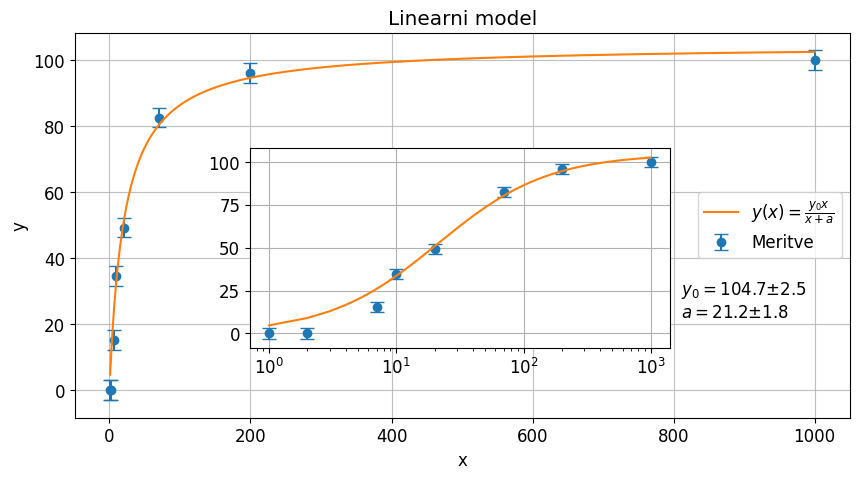
\includegraphics[width=13cm]{farma3.png}
\caption{Enačba (3) z optimalnimi parametri in točke iz tabele 1.}
\end{figure}

\subsection{Nelinearni model}

Za funkcijo, ki opisuje lahko vzamemo tudi nekaj nelinearnega kot na primer

\begin{equation}
y = \frac{y_0 x^p}{x^2 + a^p},
\end{equation}
kar pomeni, da imamo sedaj opravka z enim parametrom več. Te enačbe nemoremo linearizirati, zato lahko samo slepo zaupamo algoritmu najmanjših kvadratov oz. minimizacije $\chi^2$. Na sliki 4 lahko vidimo prileganje nelinearne krivulje našim meritvam.

\begin{figure}[h!]
\centering
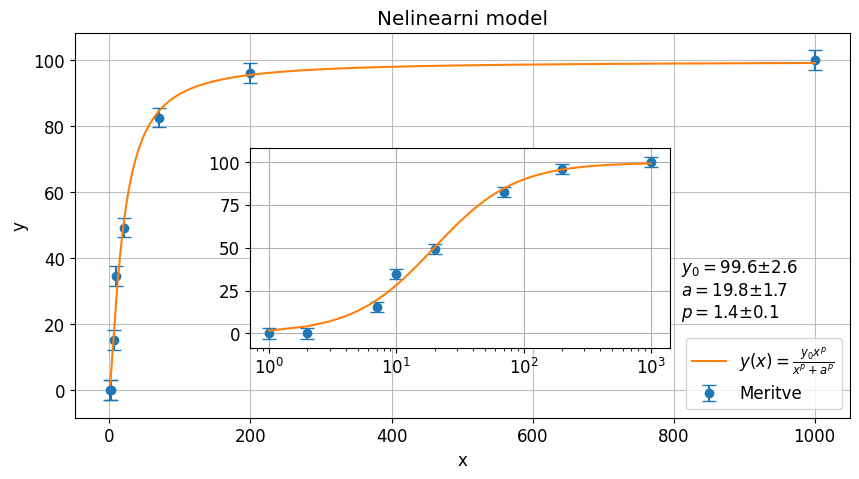
\includegraphics[width=13cm]{farma4.png}
\caption{Enačba (7) z optimalnimi parametri in točke iz tabele 1.}
\end{figure}

Želimo statistično upravičiti vpeljavo dodatnega parametra $p$. To lahko storimo s prikazom korelacijske matrike. Če korelacijski koeficient med $p$ in drugimi parametri funkcije, ki jo prilagajamo, po absolutni vrednosti ni blizu 1 parameter $p$ ni nepotreben. Na sliki 5 je prikazana korelacijska matrika in vidimo, da je upeljava $p$ upravičena.

\begin{figure}[h!]
\centering
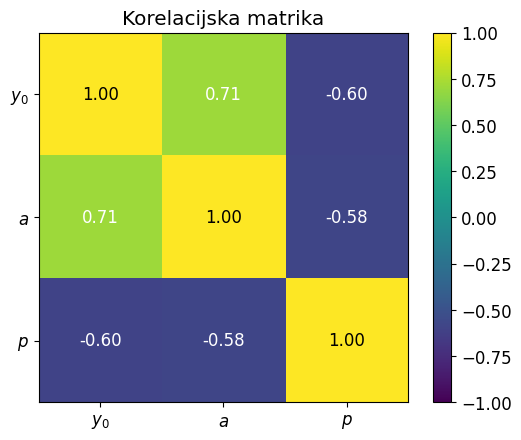
\includegraphics[width=8cm]{farma5.png}
\caption{Korelacijska matrika za parametre $y_0$, $a$ in $p$ pri nelinearnem modelu.}
\end{figure}

\subsection{Primerjava linearnega in nelinearnega modela}

Na sliki 6 lahko vidimo primerjavo obeh modelov. Nelinearni model se na prvi pogled točkam bolje prilega kot enostavnejši linearni, kar sploh lepo vidimo na grafu z logaritemsko skalo v x osi.

\begin{figure}[h!]
\centering
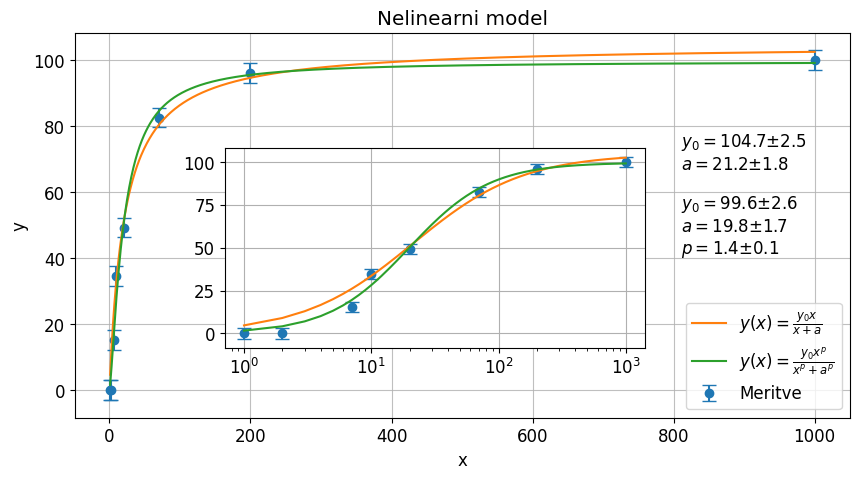
\includegraphics[width=13cm]{farma6.png}
\caption{Enačba (7) z optimalnimi parametri in točke iz tabele 1.}
\end{figure}

Dobra mera za kvaliteto modela je vrednosti reduciranega $\chi^2$ podanega z enačbo (1). Za obe dve obliki funkcij sta vrednosti reduciranega $\chi^2$ enaki
 
\[
\chi^2_{lin} = 4.35 \quad \text{ter} \quad \chi^2_{nelin} = 1.87.
\]
Vidimo, da je vrednost manjša za nelinearni model, kar nakazuje na to da je za dan primer najverjetneje boljši.

\section{Delovanje ledvic}

Iščemo najboljšo vrednost za čistilnost ledvic iz kliničnih podatkov v datoteki \texttt{ledvice.dat} na spletni učilnici. V datoteki so podani podatki o času $t$ in število sunkov na detektorju $N$. Čas je podan kot čas na sredi vsakega merilnega intervala. O napakah meritev števila sunkov ni podatka, ampak sem napako pripisal sam in sicer po Poisonnu $\sigma_N = \sqrt{N}$. Pristopili bomo z enorazdelčnim, dvorazdelčnim in bolj zapletenim modelom. Meritve iz datoteke so prikazane na sliki 7.

\begin{figure}[h!]
\centering
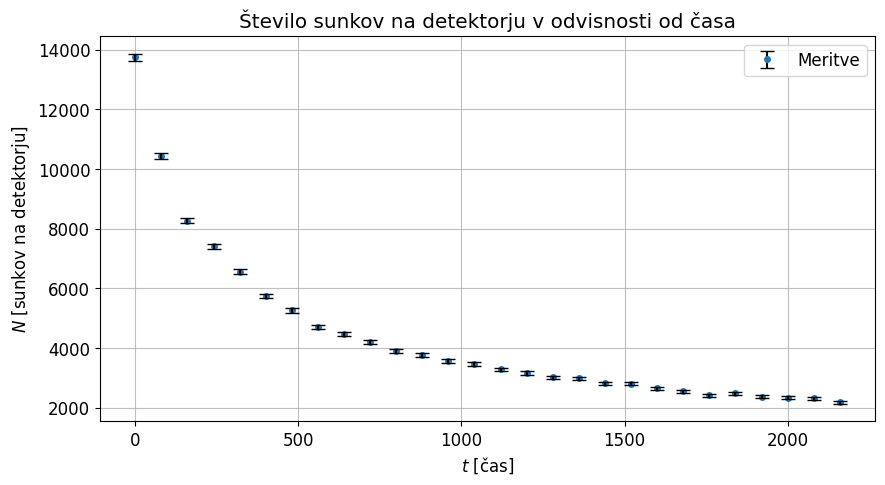
\includegraphics[width=13cm]{ledvice1.png}
\caption{Klinične meritve iz datoteke \texttt{ledvice.dat}.}
\end{figure}

\subsection{Enorazdelčni model}

Začnimo z enorazdelčnim modelom. Modelska funkcija je v tem primeru 

\begin{equation}
N(t) = Ae^{-at},
\end{equation}
kjer sta $A$ in $a$ neznana parametra. Zaradi enostavnosti funkcije lahko model lineariziramo in problem prevedemo na prilagajanje linearne funkcije čez transformirane meritve. Enačbo (8) logaritmiramo in uvedemo nove spremenljivke

\[
\tilde{N}(t) = \ln(N(t)) \quad \text{in} \quad \tilde{A} = \ln(A).
\]
Na ta način se enačba (8) prepiše v linearni funkcijo

\begin{equation}
\tilde{N}(t) = -at + \tilde{A}.
\end{equation}
Nesmemo pa pozabiti na transformacijo kliničnih podatkov in njihovih napak. V našem primeru se napake trensformirajo kot

\[
\sigma_{\tilde{N}i} = \frac{\sigma_{Ni}}{N_i} = \frac{1}{\sqrt{N_i}}.
\]
Slika 8 prikazuje linearno regresijo linearne funkcije čez linearizirane klinične podatke in optimalne parametre zanjo. 

\begin{figure}[h!]
\centering
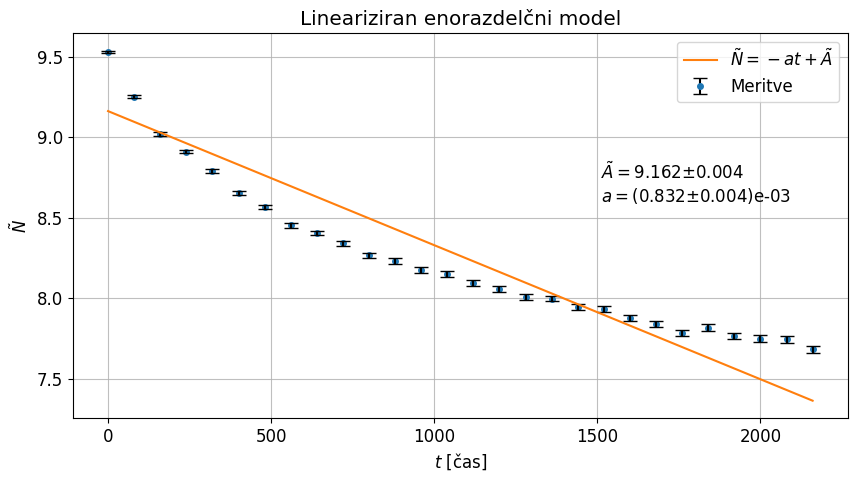
\includegraphics[width=13cm]{ledvice2.png}
\caption{Lineariziean enorazdelčni model ledvice, ki ga opiše enačba (9) z optimalnimi parametri $\tilde{A}$ in $a$.}
\end{figure}
 Iz določenih optimalnih parametrov premice lahko nato izračunamo optimalna parametra $A$ in $a$ iz enačbe (8). Na sliki 9 lahko vidimo enodelčni model ledvice, ki ga opiše enačba (8) z izračunanimi optimalnimi parametri $A$ in $a$. Krivulja se meritvam ne prilega najbolje in vrednost reduciranega $\chi^2$ je precej velika, in sicer
 
\[
\chi^2 = 169.9.
\]
To vrednost lahko zmanjšamo z bolj kompleksnimi modeli, kot na primer dodajanje aktivnosti ozadja enorazdelčnemu modelu.

\begin{figure}[h!]
\centering
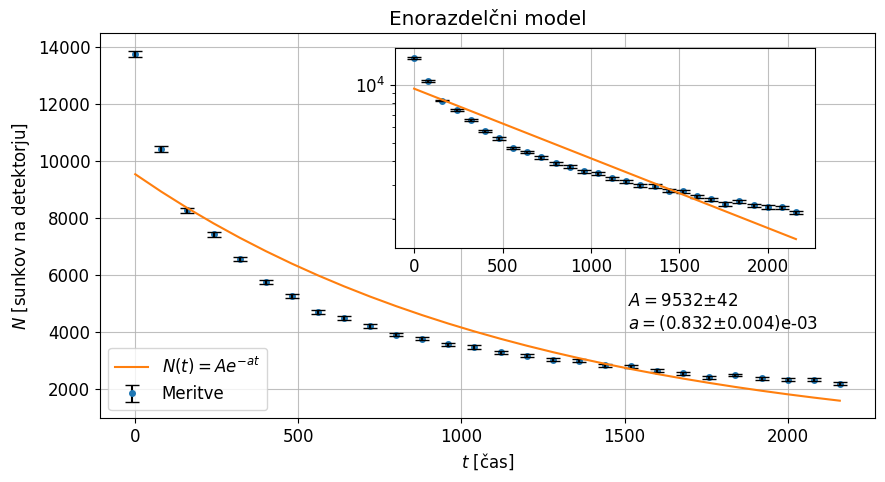
\includegraphics[width=13cm]{ledvice3.png}
\caption{Enorazdelčni model ledvice, ki ga opiše enačba (8) z optimalnimi parametri $A$ in $a$.}
\end{figure}

\subsubsection{Enorazdelčni model z ozadjem}

Enorazdelčni model lahko v tem podpodpoglavju lahko hitro izboljšamo z dodatkom sevanja ozadja $C$ v modelsko funkcijo

\begin{equation}
N(t) = Ae^{-at} + C.
\end{equation}
V tem primeru funkcije nemoremo linearizirati in kar zaupajmo \texttt{Python}-ovi funkciji \texttt{curve\_fit}. Rezultati regresije funkcije podane z enačbo (10) čez klinične podatke so prikazani na sliki 10.

\begin{figure}[h!]
\centering
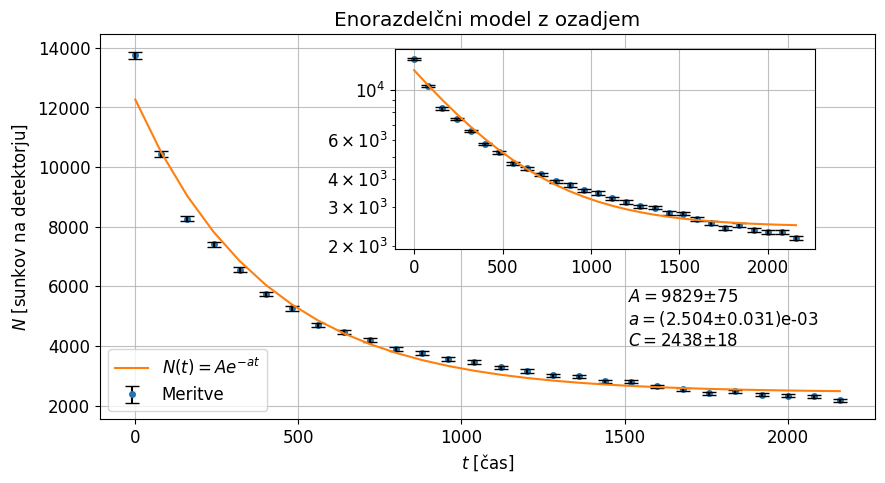
\includegraphics[width=13cm]{ledvice4.png}
\caption{Enorazdelčni model ledvice z ozadjem, ki ga opiše enačba (10) z optimalnimi parametri $A$, $a$ in $C$.}
\end{figure}
Vidimo, da se rep funkcije v tem primeru veliko bolje prilega kliničnem podatkom. Tudi vrednost reduciranega $\chi^2$ je pri tem modelu nižja kot v modelu brez ozadja, in sicer

\[
\chi^2 = 20.9.
\]
To vrednost bomo v naslednjih modelih še izboljšali. Na sliki 11 je prikazana korelacijska matrika med parametri $A$, $a$ in $C$.

\begin{figure}[h!]
\centering
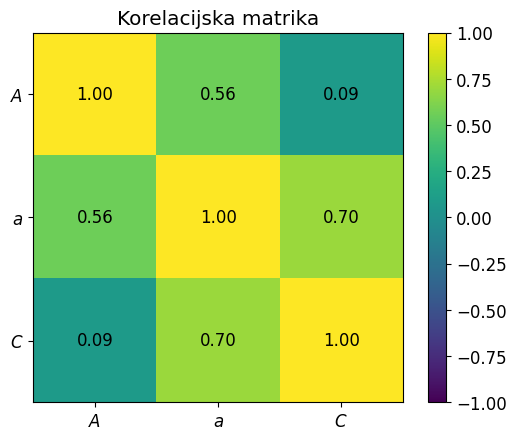
\includegraphics[width=7cm]{ledvice5.png}
\caption{Korelacijska matrika med parametri $A$, $a$ in $C$ pri enorazdelčni model ledvice z ozadjem, ki ga opiše enačba (10).}
\end{figure}

\subsection{Dvorazdelčni model}

Dvorazdelčni model opišemo z modelsko funkcijo

\begin{equation}
N(t) = Ae^{-at} + Be^{-bt}.
\end{equation}
V tem primeru imamo dve padajoči eksponentni funkciji in funkcije nemoremo linearizirati. Prilagojena funkcija z optimalnimi parametri je prikazana na sliki 11.

\begin{figure}[h!]
\centering
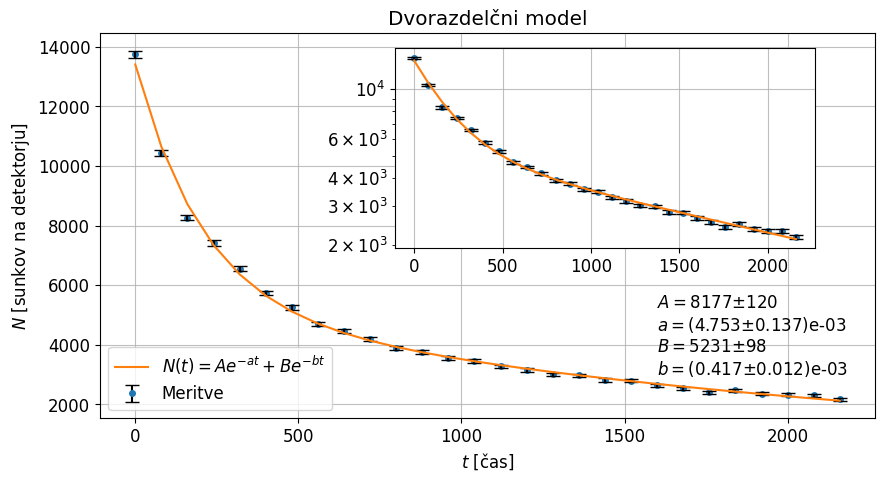
\includegraphics[width=13cm]{ledvice6.png}
\caption{Dvorazdelčni model ledvice, ki ga opiše enačba (11) z optimalnimi parametri $A$, $a$, $B$ in $b$.}
\end{figure}
Vidimo, da se funkcija bolje prilega podatkom, kot funkcija, ki opisuje enorazdelčni model. Tudi vrednost reduciranega $\chi^2$ pade na

\[
\chi^2 = 3.0,
\]
kar je bolje. Vseeno model lahko izboljšamo še z dodatkom ozadja, saj slutimo, da je sevanje ozadja prisotno. Na sliki 13 je prikazana korelacijska metrika za parametre $A$, $a$, $B$ in $b$. Vidimo, da nobena izmed parametrov nista popolno korelirana in e prisotnost vseh pomembna. Opazimo pa, da je korelacija med $B$ in $b$ vseeno precej visoka.

\begin{figure}[h!]
\centering
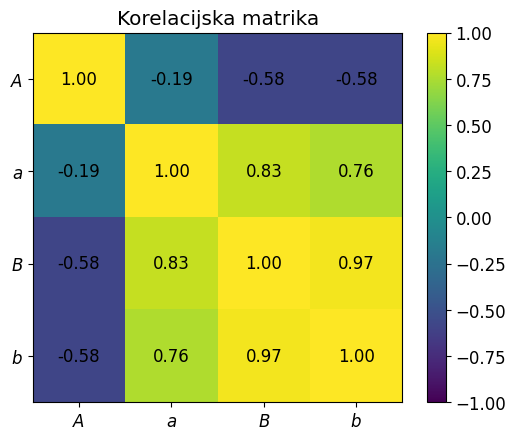
\includegraphics[width=7cm]{ledvice7.png}
\caption{Korelacijska matrika med parametri $A$, $a$, $B$ in $b$ pri dvorazdelčnem modelu ledvice, ki ga opiše enačba (11).}
\end{figure}

\subsubsection{Dvorazdelčni model z ozadjem}

Dvorazdelčni model lahko hitro še bolj izboljšamo z dodatkom sevanja ozadja. Tako modelski funkciji prištejemo še neko konstantno vrednost $C$, ki predstavlja konstantno sevanje ozadja

\begin{equation}
N(t) = Ae^{-at} + Be^{-bt} + C.
\end{equation}
Funkcija iz enačbe (12) prilagojena podatkom je prikazana na sliki 14.

\begin{figure}[h!]
\centering
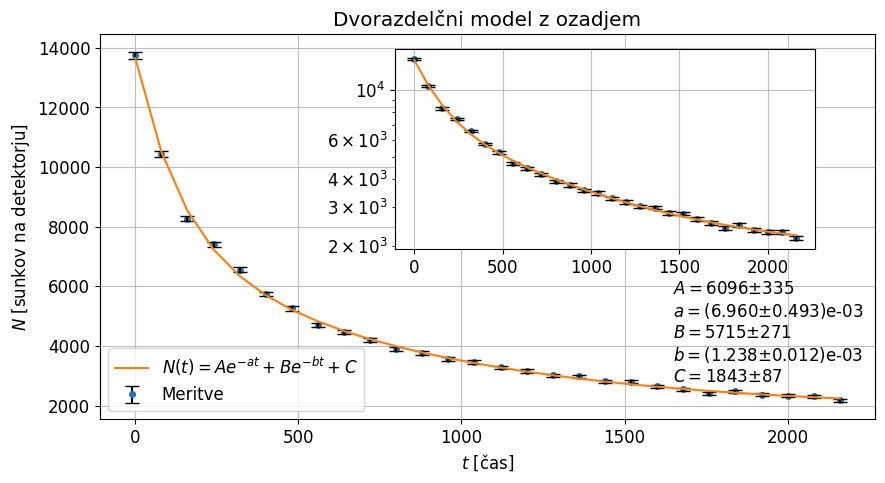
\includegraphics[width=13cm]{ledvice8.png}
\caption{Dvorazdelčni model ledvice z ozadjem, ki ga opiše enačba (12) z optimalnimi parametri $A$, $a$, $B$, $b$ in $C$.}
\end{figure}
Vidimo, da se prilagojena funkcija lepo ujema s izmerki. V tem primeru vrednosti reduciranega $\chi^2$ doseže

\[
\chi^2 = 1.7,
\]
kar nakazuje na to, da je dvorazdelčni model z ozadjem zelo dober. Korelacijska matrika na sliki 15 pokaže tudi, da noben izmed parametrov ni popolnoma koreliran in imajo v obliki krivulje vsi svojo vlogo.

\begin{figure}[h!]
\centering
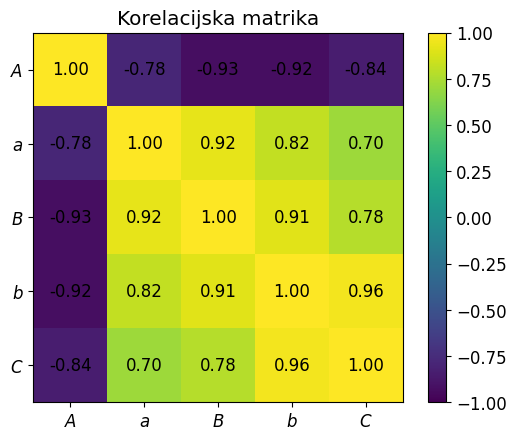
\includegraphics[width=7cm]{ledvice9.png}
\caption{Korelacijska matrika med parametri $A$, $a$, $B$, $b$ in $C$ pri dvorazdelčnem modelu ledvice z ozadjem, ki ga opiše enačba (12).}
\end{figure}

\subsection{Zapleten model}

V nalogi je omenjeno, da lahko poskusimo modelirati delovanje ledvic tudi z bolj zapleteno funkcijo, ki ima v eksponentih korene časa

\begin{equation}
N(t) = Ae^{-a\sqrt{t}} + Be^{-b\sqrt{t}} + C.
\end{equation}
To funkcijo priležemo podatkom in dobimo rezultat na sliki 16.

\begin{figure}[h!]
\centering
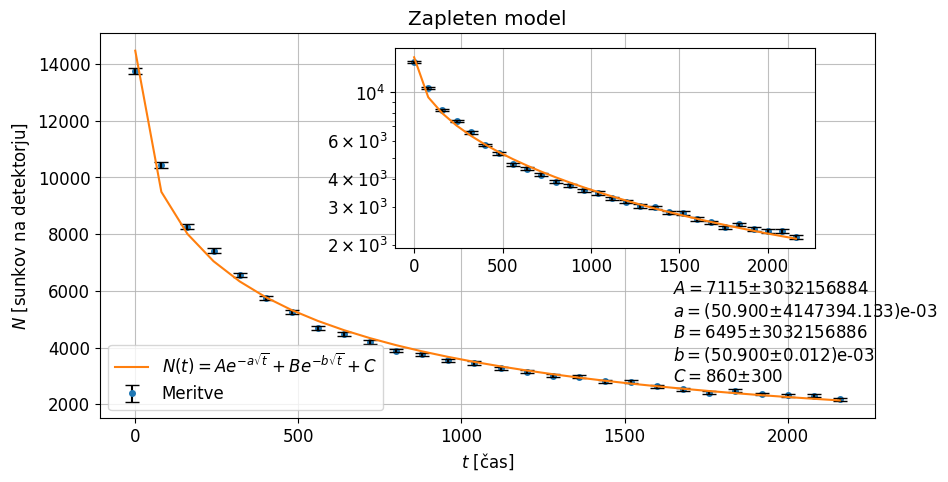
\includegraphics[width=13cm]{ledvice10.png}
\caption{Zapleten model ledvice, ki ga opiše enačba (13) z optimalnimi parametri $A$, $a$, $B$, $b$ in $C$.}
\end{figure}
Vidimo, da se sicer krivulja lepo prilega podatkom, a napake parametrov so ogromne. Vrednost reduciranega $\chi^2$ je v tem primeru enaka

\[
\chi^2 = 9.3,
\]
kar je boljše kot v enorazdelčnem modelu a slabše kot v dvorazdelčnem. Na sliki 17 vidimo korelacijsko matriko in opazimo razlog za ogromne napake nekaterih parametrov na sliki 16. Absolutna vrednost korelacijskega koeficienta med nekaterimi parametri je enaka oziroma je zelo blizu 1, in sicer med parametroma $A$ in $B$ ter med parametroma $a$ in $b$. To pomeni, da lahko v modelski funkciji odstranimo enega izmed parametrov v vsakem paru in tako reduciramo ta zapleten model.

\begin{figure}[h!]
\centering
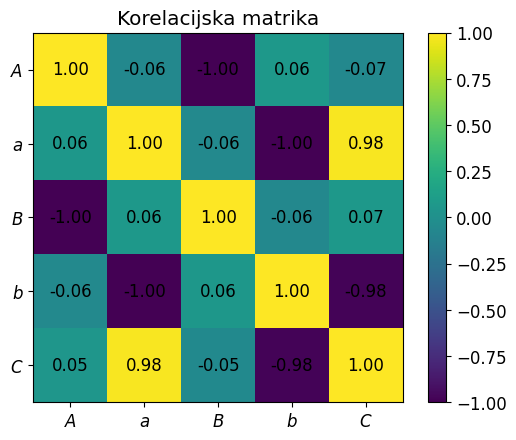
\includegraphics[width=7cm]{ledvice11.png}
\caption{Korelacijska matrika med parametri $A$, $a$, $B$, $b$ in $C$ pri zapletenem modelu ledvice z ozadjem, ki ga opiše enačba (13).}
\end{figure}

\subsubsection{Reducirani zapleten model}

Zapleteni model zgoraj lahko zaradi popolne antikorelacije med določenimi parametri reduciramo do nove reducirane modelske funkcije

\begin{equation}
N(t) = Ae^{-a\sqrt{t}} + C.
\end{equation}
Tako smo se izognili nepotrebnim komplikacijam z nepotrebnimi parametri. To funkcijo nato prilegamo kliničnim podatkom. Rezultati so prikazani na sliki 18.

\begin{figure}[h!]
\centering
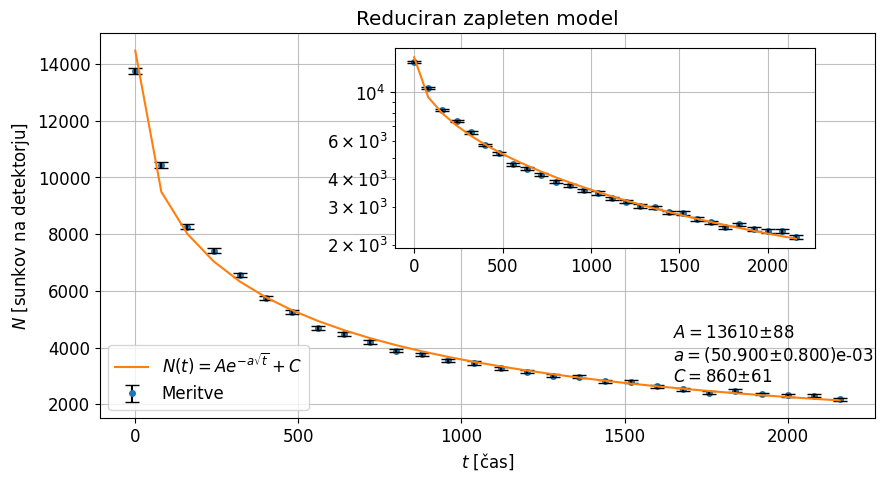
\includegraphics[width=13cm]{ledvice12.png}
\caption{Reducirani zapleten model ledvice, ki ga opiše enačba (14) z optimalnimi parametri $A$, $a$ in $C$.}
\end{figure}
Vidimo, da se krivulja mepo prilagaja meritvam. Vrednost reduciranega $\chi^2$ je enaka

\[
\chi^2 = 8.5,
\]
ker je bolje kot prej. Na sliki 19 vidimo tudi korelacijsko metriko med koeficienti $A$, $a$ in $C$, ki kaže to, da smo se znebili popolnoma koreliranih ali antikoreliranih parametrov. Znebili smo se nepotrebnih komplikacij.

\newpage

\begin{figure}[h!]
\centering
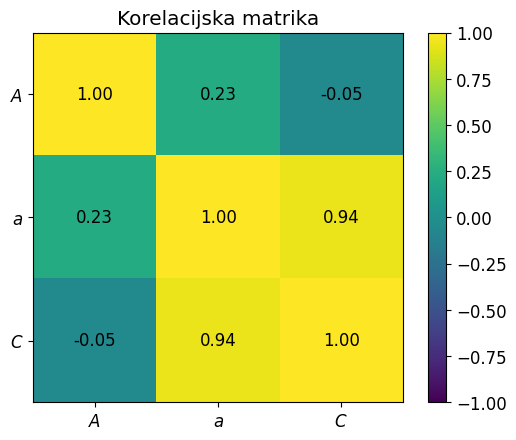
\includegraphics[width=7cm]{ledvice13.png}
\caption{Korelacijska matrika med parametri $A$, $a$ in $C$ pri reduciranem zapletenem modelu ledvice z ozadjem, ki ga opiše enačba (14).}
\end{figure}

\subsection{Primerjava modelov}

Vse modele na preprost način primerjam po vrednosti reduciranega $\chi^2$ prikazane v tabeli 3. V tem primeru je najboljši model tudi model z največ parametri, in sicer dvorazdelčni model ledvice z ozadjem. Največjo vrednost reduciranega $\chi^2$ pa ima preprost enorazdelčni model.

\begin{table}[h!]
\centering
\begin{tabular}{ccr}
\toprule
                 Model &      $\chi^2$ \\
\midrule
          Enorazdelčni &  169.9 \\
Enorazdelčni z ozadjem &   20.9 \\
          Dvorazdelčni &    3.0 \\
Dvorazdelčni z ozadjem &    1.7 \\
              Zapleten &    9.3 \\
    Reduciran zapleten &    8.5 \\
\bottomrule
\end{tabular}
\caption{Vrednosti $\chi^2$ za različne modele ledvice.}
\end{table}

\section{Magnetni spektrometer}

Za uporabo visokoločljivega magnetnega spektrometra potrebujemo preslikavo, ki iz izmerjenih količin rekonstruira parametre trajektorije delcev, potrebne za izračun energije in drugih kinematičnih količin. Iz datoteke \texttt{thtg-xfp-thfp.dat} preberemo $\theta_{tg}$ (disperzijski kot na tarči v stopinjah) ter $x_{fp}$ (položaj v goriščni ravnini v milimetrih) in $\theta_{fp}$ (kot v goriščni ravnini v stopinjah). Zanima nas varčni model za preslikavo

\begin{equation}
(x_{fp}, \theta_{fp}) \rightarrow \theta_{tg}.
\end{equation}
Na sliki 20 so prikazani podatki iz datoteke.

\begin{figure}[h!]
\centering
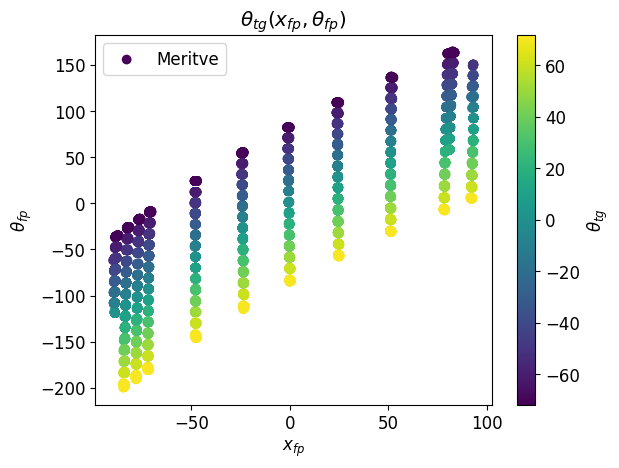
\includegraphics[width=10cm]{spektro1.png}
\caption{Elementi matrik $A$, $U$, $W$ in $V^T$.}
\end{figure}

Sestavili bomo model, ki vsebuje potence $x_{fp}$ in $\theta_{fp}$. Neznani parametri, ki jih bomo poiskali z SVD razcepom so koeficienti pred členi $x_{fp}^n \theta_{fp}^m$. Model je

\begin{equation}
\theta_{tg} = \sum_k a_k a_{fp}^{n_k} \theta_{fp}^{m_k},
\end{equation}
kjer si potence sledijo kot

\begin{equation}
L = [(0,0), (1,0), (0,1), (2,0), (1,1), (0,2), ..., (n_k, m_k), ...].
\end{equation}
V vsoti oz. modelu, ki ga opiše enačba (16) vzamemo prvim $M$ členov, kar pomeni, da imamo $M$ neznanih parametrov. Za reševanje problema linearne minimizacije kvadratov si bomo pomagali s SVD razcepom

\begin{equation}
A = UWV^T,
\end{equation}
kjer je matrika $A$ enaka

\begin{equation}
A = [1 \quad x_{fp} \quad \theta_{fp} \quad x_{fp}^2 \quad x_{fp}\theta_{fp} \quad \theta_{fp}^2 \quad ... ].
\end{equation}
Po receptu je nato vektor optimalnih parametrov, ki ga iščemo, enak

\begin{equation}
\textbf{a} = \sum_i^M \left( \frac{\textbf{U}_i \cdot \textbf{b}}{w_i} \right) \textbf{V}_i,
\end{equation}
kjer je $\textbf{b} = [\theta_{tg}]$. Kovarianca in seveda tudi varianca pa je podana s formulo

\begin{equation}
\text{cov}[a_j, a_k] = \sum_{i=1}^M \frac{V_{i,j} V_{i,k}}{w_i^2}.
\end{equation}

Za primer si oglejmo model v katerem v modelski funkciji, ki jo podaja enačba (16), vzamemo vse člene dokler vsota potenc ni večja kot 10. Na sliki 21 so prikazani elementi matrik $A$, $U$, $W$ in $V^T$. Na sliki 22 pa je prikazana rešitev $a$ pridobljena po enačbi (20) ter kovariančna matrika med parametri pridobljena po enačbi (21).V korelacijski matriki vidimo velike korelacije med določenimi parametri. Sploh pri parametrih desno spodaj. Za napako meritev vzamemo $0.3^\circ$ in tako dobimo za ta model vrednost reduciranega $\chi^2$ enako

\[
\chi^2 = 1.9.
\]

\begin{figure}[h!]
\centering
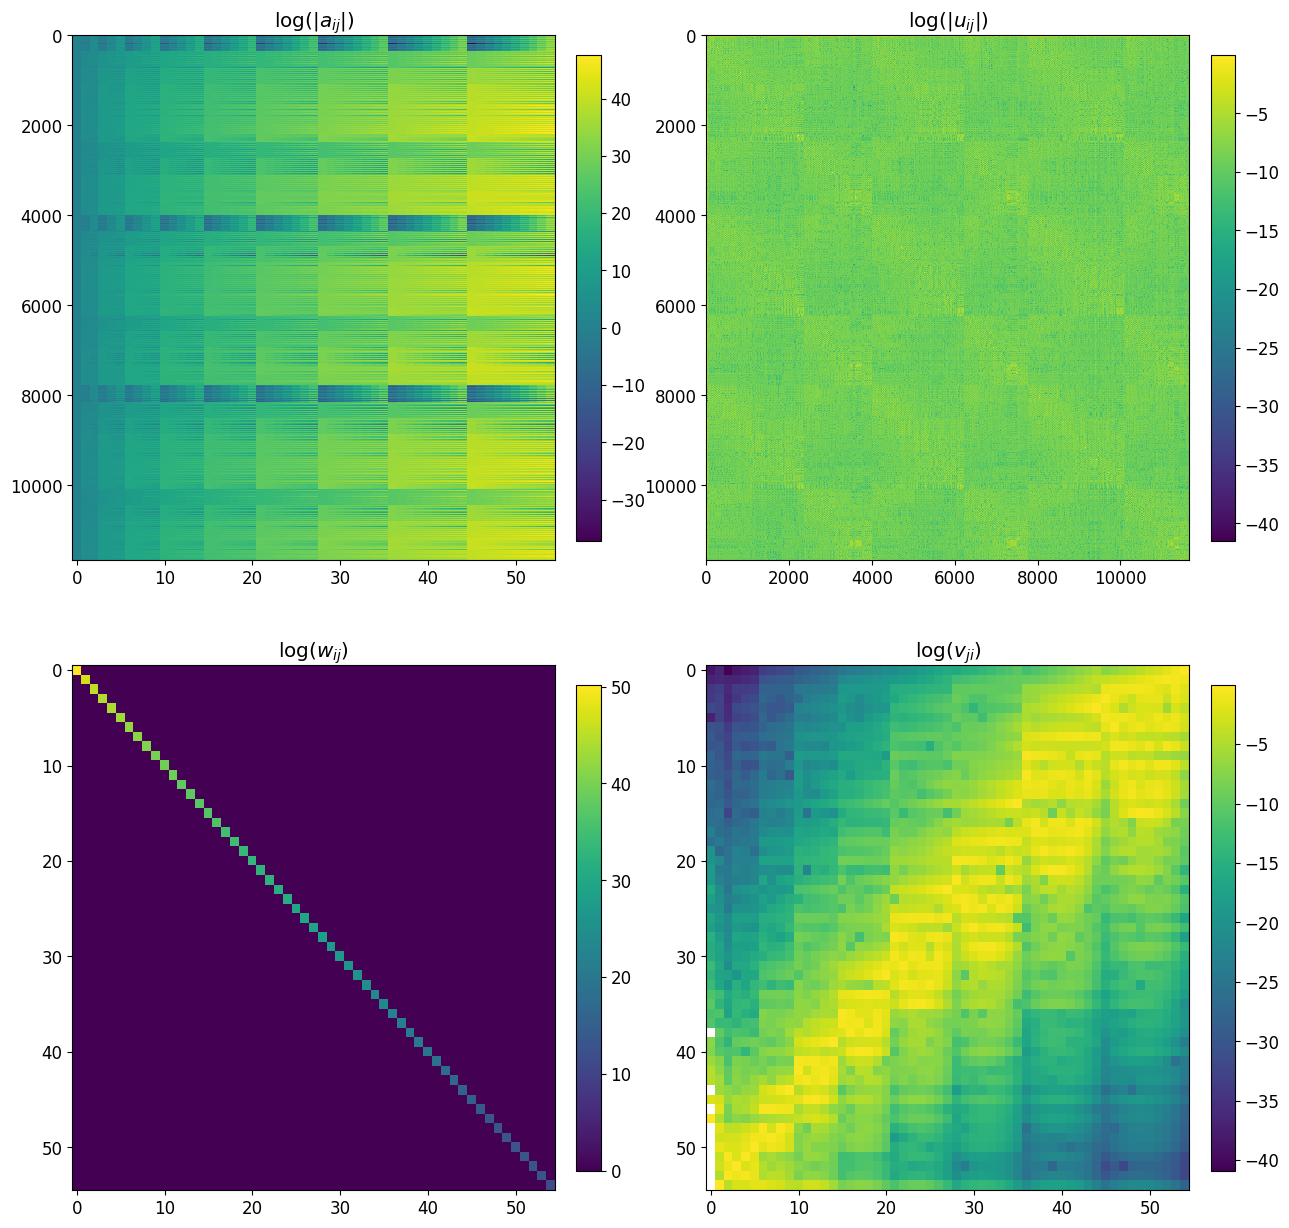
\includegraphics[width=14cm]{spektro2.png}
\caption{Elementi matrik $A$, $U$, $W$ in $V^T$.}
\end{figure}

\begin{figure}[h!]
\centering
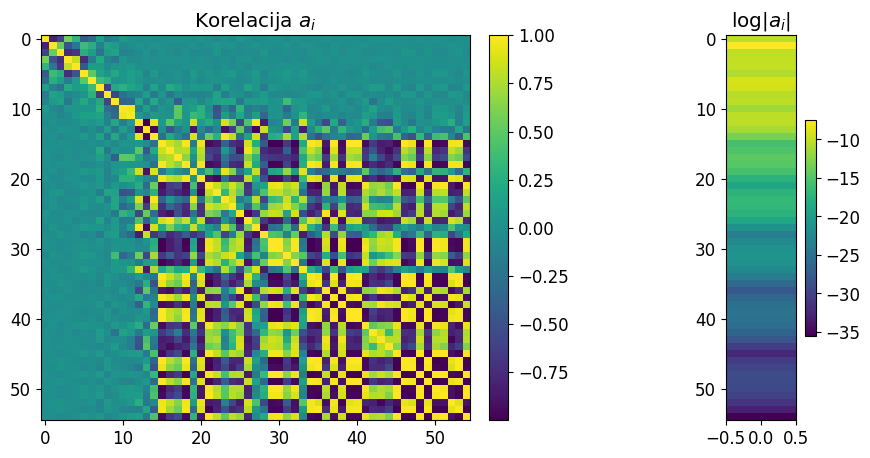
\includegraphics[width=14cm]{spektro3.png}
\caption{Elementi vektorja $\textbf{a}$ ter kovariančne matrike med parametri modela.}
\end{figure}

Na sliki 23 lahko vidimo vrednost reduciranega $\chi^2$ v odvisnosti od števila parametrov $M$. Sumljivo je, da se na začetku in kasneje po 500 parametrih vrednost reduciranega $\chi^2$ viša skupaj s številom parametrov. Razloga za to ne poznam, saj sem skozi napisano kodo šel večkrat in napake nisem videl.

Študijo o tem modelu bi lahko še nadaljeval tako, da bi luščil iz vseh parametrov le tiste najbolj potrebne. To bi storil na način, da bi izločil enega v paru med seboj popolno koreliranih parametrov. Na sliki 22 vidimo, da je teh parametrov veliko in sklepam, da je pri večjem parametru takšnih parov še več. Žal mi zaradu časovne stiske to ni uspelo.

\begin{figure}[h!]
\centering
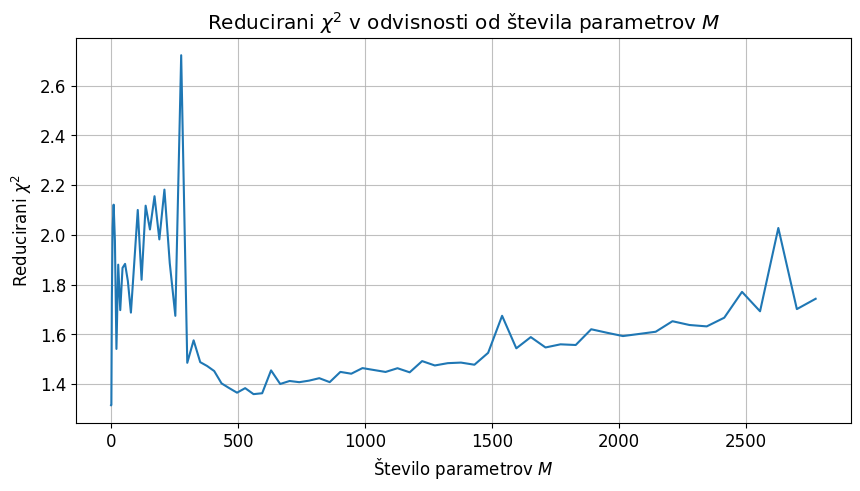
\includegraphics[width=13cm]{spektro4.png}
\caption{Vrednost reduciranega $\chi^2$ v odvisnosti od števila parametrov v modelu.}
\end{figure}

\section{Zaključek}

Spoznali smo linearno minimizacijo kvadratov in vrednost $\chi^2$ na treh različnih modelih. Z obravnavo prvih dveh delov naloge sem zadovoljen, za podrobnejšo obravnavo tretjega dela pa mi je žal zmanjkalo nekaj časa.

\end{document}